% CE7454 Project 1 report -- built on the official CVPR 2026 author kit (camera-ready style)
\documentclass[10pt,twocolumn,letterpaper]{article}
\usepackage{cvpr}
%% This file contains a number of tweaks that are typically applied to the main document.
%% They are not enabled by default, but can be enabled by uncommenting the relevant lines.

%%
%% Inline annotations; for predefined colors, refer to "dvipsnames" in the xcolor package:
%% https://tinyurl.com/overleaf-colors
%%
\newcommand{\red}[1]{{\color{red}#1}}
\newcommand{\todo}[1]{{\color{red}#1}}
\newcommand{\TODO}[1]{\textbf{\color{red}[TODO: #1]}}
%%
%% disable for camera ready / submission by uncommenting these lines  
%%
% \renewcommand{\TODO}[1]{}
% \renewcommand{\todo}[1]{#1}

%%
%% work harder in optimizing text layout. Typically shrinks text by 1/6 of page, enable
%% it at the very end of the writing process, when you are just above the page limit
%%
% \usepackage{microtype}

%%
%% fine-tune paragraph spacing
%%
% \renewcommand{\paragraph}[1]{\vspace{.5em}\noindent\textbf{#1.}}

%%
%% globally adjusts space between figure and caption
%%
% \setlength{\abovecaptionskip}{.5em}


%%
%% Allows "the use of \paper to refer to the project name"
%% with automatic management of space at the end of the word
%%
% \usepackage{xspace}
% \newcommand{\paper}{ProjectName\xspace}

%%
%% Commonly used math definitions
%%
% \DeclareMathOperator*{\argmin}{arg\,min}
% \DeclareMathOperator*{\argmax}{arg\,max}

%%
%% Tigthen underline
%%
% \usepackage{soul}
% \setuldepth{foobar}
\usepackage{booktabs}
\usepackage{microtype}
\graphicspath{{../figures/}}
\setlength{\abovecaptionskip}{0.3em}
\raggedbottom
\setlength{\textfloatsep}{0.7em plus 0.2em minus 0.2em}
\setlength{\dbltextfloatsep}{0.7em plus 0.2em minus 0.2em}
\renewcommand{\paragraph}[1]{\vspace{0.2em}\noindent\textbf{#1.}}
\definecolor{cvprblue}{rgb}{0.21,0.49,0.74}
\usepackage[pagebackref=false,breaklinks,colorlinks,allcolors=cvprblue]{hyperref}
\newcommand{\codeurl}{https://github.com/Vrushank-Ahire/CE7454-Project1}

\def\paperID{CE7454-P1}
\def\confName{CVPR}
\def\confYear{2026}

\title{DSR-Net: A Dual-Stream RGB--Residual CNN for AI-Generated Image\\Attribution, and Why It Failed under Test-Set Shift}

\author{Ahire Vrushank Ajay\quad(G2608495L)\\
College of Computing and Data Science, Nanyang Technological University, Singapore\\
CE7454 Deep Learning for Data Science, Project 1\\
{\small Code: \href{\codeurl}{\texttt{github.com/Vrushank-Ahire/CE7454-Project1}}}
}

\begin{document}
\maketitle

%---------------------------------------------------------------------------
\begin{abstract}
We classify $512{\times}512$ JPEG images as real or as produced by one of two undisclosed generators, under a 12.3M-parameter budget with training from scratch on the 15,000 supplied images. DSR-Net is a 7.79M-parameter CNN that fuses an RGB branch with a branch fed by fixed SRM-style high-pass residuals, trained on JPEG-grid-aligned crops with JPEG re-encoding augmentation. It scores 0.991 on a held-out training split and 0.979 on the development set, but 0.484 on the hidden test set, where it predicts Model B for only 21 of 1,500 images. We report this gap as the main result, separate what the prediction files prove from what they cannot, and show that our validation protocol measured only in-distribution accuracy.
\end{abstract}

%---------------------------------------------------------------------------
\section{Problem and data}
\label{sec:intro}
Each image has a label $y\in\{0,1,2\}$ (real, Model A, Model B), so the task joins real/fake detection with source attribution~\cite{yu2019attributing}. The rules forbid pretrained weights, external data, ensembles, test-time augmentation and distillation. The training set has 5,000 images per class; dev (900) and test (1,500) labels are hidden and scored on CodaBench.

\paragraph{Supplied samples: observed vs.\ inferred}
\Cref{fig:data} shows the twelve supplied samples. We \emph{observe} that: (i) all twelve are $512{\times}512$ baseline JPEGs with identical IJG quality-95 tables and 4:2:0 chroma subsampling; (ii) within a scene, the three images share subject, objects and layout, but the generated ones change pose and viewpoint and are not pixel-aligned with the photograph; (iii) the photographs carry phone-filter vignetting and grading, while the generated images look cleaner and more saturated; (iv) one real file keeps an \texttt{AppleMark} JPEG comment from its source. We \emph{infer}, without being able to verify, that the generated images came from text-to-image synthesis conditioned on a description of the photograph, and that all classes were then resized and re-encoded to a common format. Scene semantics therefore carry little label information. A detector has to rely on low-level traces and on each class's processing history, which is where shortcut cues and fragility to post-processing are known risks~\cite{grommelt2024fake,geirhos2020shortcut}. DSR-Net reads decoded pixels only, so metadata such as (iv) is unused.

\begin{figure}[t]
  \centering
  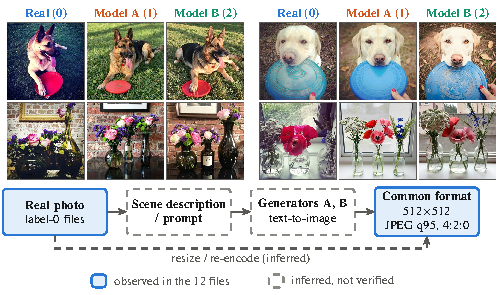
\includegraphics[width=\linewidth]{dataset.pdf}
  \caption{The twelve supplied training samples (four scenes $\times$ three classes) and our reading of the generation pipeline. Blue solid boxes are observed in the files; grey dashed boxes and arrows are inferred.}
  \label{fig:data}
\end{figure}

%---------------------------------------------------------------------------
\section{Related work}
\label{sec:related}
Wang \etal~\cite{wang2020cnn} showed that a ResNet-50 trained on one GAN with blur and JPEG augmentation transfers to other CNN generators. Frank \etal~\cite{frank2020leveraging} traced detectability to spectral up-sampling artefacts, and Tan \etal~\cite{tan2024rethinking} model local up-sampling correlations directly. Yu \etal~\cite{yu2019attributing} attribute images to individual GANs through learned fingerprints, the analogue of our A-vs-B decision. Corvi \etal~\cite{corvi2023detection} found that GAN-trained detectors transfer poorly to diffusion models and degrade on resized and compressed images. Ojha \etal~\cite{ojha2023towards} generalise better with frozen CLIP features, which the rules exclude here. Spatial rich models~\cite{fridrich2012rich} suppress content with fixed high-pass filters and truncate the residuals. Zhou \etal~\cite{zhou2018learning} pair an RGB stream with an SRM stream for manipulation detection, and Bayar and Stamm~\cite{bayar2016deep} learn such filters with a constrained layer. DSR-Net is a compact, from-scratch classification version of the RGB+SRM design of~\cite{zhou2018learning}, not a new principle. On bias and shift, Gragnaniello \etal~\cite{gragnaniello2021gan} showed that resizing and compression in training and testing govern how well detectors generalise. GenImage~\cite{zhu2023genimage} tests on unseen generators and degraded images, and Grommelt \etal~\cite{grommelt2024fake} found that GenImage detectors partly learn JPEG format and image size. Removing these biases raised cross-generator accuracy by about 11 points.

%---------------------------------------------------------------------------
\begin{figure*}[t]
  \centering
  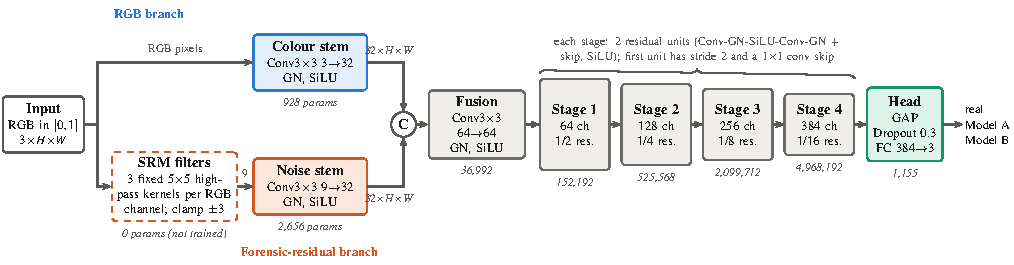
\includegraphics[width=\textwidth]{architecture.pdf}
  \caption{DSR-Net (\texttt{DualStreamForensicNet} in \texttt{aigi\_jpeg.py}). The input is split into an RGB branch and a forensic-residual branch. The branches are fused at full resolution, and their combined features pass through four residual stages to a three-way classifier. Italic numbers are trainable parameters per block, computed from layer shapes; they sum to the 7,787,395 printed in the training log (limit 12.3M). The dashed SRM block is fixed. C: channel concatenation (64 channels); GN: GroupNorm (8 groups); GAP: global average pooling. Spatial size is unchanged until Stage~1 (training crops $H{=}W{=}256$; inference on full images).}
  \label{fig:arch}
\end{figure*}

\section{Method}
\label{sec:method}
\paragraph{Architecture (\cref{fig:arch})}
The input is RGB in $[0,1]$, with no mean/std normalisation. The \emph{forensic branch} filters each colour channel with three fixed $5{\times}5$ kernels: the zero-padded $3{\times}3$ second-order ``square'' kernel ($/4$), the KV kernel ($/12$)~\cite{fridrich2012rich} and a horizontal first difference $[1,-1]$. The nine residual maps are clamped to $\pm3$ and are not trained; a $3{\times}3$ convolution (9$\to$32, GroupNorm, SiLU) follows. The \emph{RGB branch} applies a parallel $3{\times}3$ convolution (3$\to$32), which keeps colour statistics such as the grading in \cref{fig:data}. Both branches stay at full resolution and are fused early (concatenation, then $3{\times}3$ 64$\to$64), so the trunk can relate residual and colour features at fine scale. Four stages of two residual units~\cite{he2016deep} (stride 2 in the first unit) widen to 64/128/256/384 channels. Global average pooling, dropout 0.3 and a linear layer give three logits. GroupNorm~\cite{wu2018group} replaces BatchNorm because inference runs one full image at a time, at a different size from the training crops.

\paragraph{Rationale and one caveat}
High-pass residuals suppress scene content, which here is shared across classes, and expose sensor noise and synthesis traces~\cite{fridrich2012rich,zhou2018learning}. No downsampling before stage 1 preserves high frequencies~\cite{frank2020leveraging}. With only 15k images, fixed filters gave a stable input. Caveat: the filters act on $[0,1]$ values rather than 8-bit values, so the $\pm3$ clamp almost never fires and the residuals are effectively untruncated, unlike~\cite{fridrich2012rich}.

\paragraph{Training and inference}
A random 5\% of the training set (750 images, seed 42) is held out; the remaining 14,250 are used for training. With probability 0.8 the \emph{full} image is re-encoded as JPEG at quality $q\sim\mathcal{U}[75,98]$. A $256^2$ crop is then taken at offsets that are multiples of 8, so it stays on the JPEG block grid, and flipped with probability 0.5. Optimisation uses cross-entropy, AdamW~\cite{loshchilov2019decoupled} (learning rate $10^{-3}$, weight decay $10^{-4}$, batch 32) and per-step cosine decay over 30 epochs (13,350 steps), in FP32 on one A100 (20.1 min). Validation uses full images re-encoded once at $q{=}91$, and the best validation checkpoint is kept. Dev and test images are classified at native size in one forward pass, with no test-time augmentation or ensembling.

%---------------------------------------------------------------------------
\section{Results}
\label{sec:exp}
\begin{figure}[t]
  \centering
  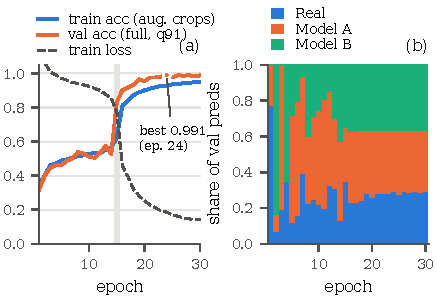
\includegraphics[width=\linewidth]{curves.pdf}
  \caption{From the job log. (a) Training loss, training accuracy on augmented crops and validation accuracy (750 images, $q{=}91$); the grey band marks the jump at epoch 15. (b) Predicted class shares on the validation split per epoch.}
  \label{fig:curves}
\end{figure}

\begin{table}[t]
  \centering\small
  \setlength{\tabcolsep}{4pt}
  \begin{tabular}{@{}lrcc@{}}
    \toprule
    Split & $n$ & Acc. & Predicted real / A / B \\
    \midrule
    Internal val ($q{=}91$) & 750 & 0.991 & 220 / 256 / 274 \\
    Dev (CodaBench) & 900 & 0.979 & 258 / 342 / 300 \\
    Test (CodaBench) & 1,500 & 0.484 & 1,011 / 468 / 21 \\
    \bottomrule
  \end{tabular}
  \caption{The single submitted model. Counts come from the log (val) and the submitted JSON files. Dev and test labels are hidden, so no confusion matrices are possible.}
  \label{tab:results}
\end{table}

\paragraph{Learning dynamics (\cref{fig:curves})}
For 14 epochs validation accuracy stays between 0.32 and 0.57, and predictions repeatedly collapse onto one or two classes (578/172/0 at epoch 1, 261/0/489 at epoch 4). Between epochs 14 and 15 it jumps from 0.528 to 0.832, while the training loss drops from 0.853 to 0.776 and then to 0.460 at epoch 16. It peaks at 0.9907 at epoch 24, the submitted checkpoint, and training-crop accuracy ends at 0.947.

\paragraph{Scores (\cref{tab:results})}
The internal split and dev agree (0.991 vs.\ 0.979), and dev predictions are spread over all classes. On test, accuracy is 0.484 and predictions are 67.4\% real, 31.2\% Model A and 1.4\% Model B.

%---------------------------------------------------------------------------
\section{Analysis: why 0.484 after 0.979?}
\label{sec:analysis}
\paragraph{Evidence (from the files)}
\textbf{E1} (\cref{fig:dist}). Model B predictions fall from 33.3\% (dev) to 1.4\% (test), and real predictions rise from 28.7\% to 67.4\%. \textbf{E2.} The shift covers the whole test set: each of the ten consecutive 150-file blocks has 0--4 Model B predictions. \textbf{E3.} At most 21 Model B images can be classified correctly, so at least 705 of the 726 correct test predictions come from real and Model A images. \textbf{E4.} If the 0.979 dev score belongs to the submitted dev file, the dev labels are not uniform: 258 real predictions against 300 real images would cap accuracy at 0.953. Test balance therefore cannot be assumed. Under a balanced test set, Model B recall would be at most 4.2\%. Without labels we cannot say which predictions are wrong, nor separate Model B images absorbed into ``real'' from a change in class priors.

\begin{figure}[t]
  \centering
  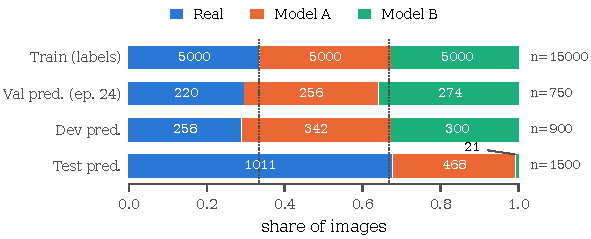
\includegraphics[width=\linewidth]{distributions.pdf}
  \caption{Class shares: training labels, and predictions on validation (epoch 24), dev and test. Dotted lines mark the 1/3 and 2/3 boundaries. Only predictions are shown for dev and test, because their labels are hidden.}
  \label{fig:dist}
\end{figure}

\paragraph{Hypotheses (not verified), with the test that would decide each}
\textbf{H1: processing shift.} Test images underwent processing absent from training and dev (resampling, a different compression chain), which erased the high-frequency cue that identifies Model B, so those images defaulted to ``real''. This drift towards ``real'' is the failure reported for processed images~\cite{corvi2023detection,gragnaniello2021gan}. The abrupt jump at epoch 15 also fits a decision built on one narrow cue. \emph{Test:} accuracy of held-out training images under rescaling and blur. \textbf{H2: format shortcut.} Real and generated images reached the common format by different routes; if the network keyed on that history~\cite{grommelt2024fake}, a differently produced test set breaks it. \emph{Test:} compare per-class and per-split quantisation and size statistics, and retrain after randomly resampling every class. \textbf{H3: generator or prompt shift.} We have no evidence either way.

\paragraph{Main limitation: validation was in-distribution}
The held-out split came from the training distribution, and given the triplet structure it probably contained scene siblings of training images. Its only difference from training was one JPEG quality inside the augmentation range. Dev turned out to be in-distribution too (0.991 vs.\ 0.979). Model selection therefore rewarded a cue whose robustness was never measured. Training-crop accuracy (0.947) is below validation accuracy, so this is a robustness failure, not ordinary overfitting. Other limitations: one seed, twelve samples for the data analysis, and no test images.

\paragraph{Priority improvements, all within the rules}
(1) Validation under transformations held out from training (0.5--1.5$\times$ resizing, blur, noise, double JPEG), plus monitoring the predicted class mix on the unlabelled test set, which would have flagged E1 before submission. (2) Augmentation with resampling, blur and noise applied to every class~\cite{wang2020cnn}. (3) Ablations: RGB vs.\ residual vs.\ both, JPEG augmentation on/off, and fixed SRM vs.\ a constrained layer~\cite{bayar2016deep}. (4) Residuals on the 8-bit scale with an active truncation threshold~\cite{fridrich2012rich}.

%---------------------------------------------------------------------------
\section{Conclusion}
DSR-Net, a compact RGB+SRM CNN trained from scratch, is nearly perfect on in-distribution data and fails on the hidden test set, where it almost never predicts Model B. The architecture follows established forensic designs. What failed was the protocol: every validation signal shared the training distribution, so a fragile cue looked like a good model.

{\small
\bibliographystyle{ieeenat_fullname}
\bibliography{refs}
}

\end{document}
